\documentclass[11pt,a4paper]{article}
\usepackage[margin=22mm]{geometry}
\usepackage[T1]{fontenc}
\usepackage[utf8]{inputenc}
\usepackage{lmodern,microtype}
\usepackage{graphicx,booktabs,tabularx,longtable,array,enumitem,xcolor,hyperref,tikz}
\usetikzlibrary{arrows.meta,positioning}
\hypersetup{colorlinks=true,linkcolor=blue!55!black,urlcolor=blue!55!black}
\setlist{nosep,leftmargin=1.5em}
\renewcommand{\arraystretch}{1.16}
\newcolumntype{Y}{>{\raggedright\arraybackslash}X}
\title{\Huge CareerCompass\\[5pt]\Large Mobile Application Design Document}
\author{DSW02B1 Group Project\\University of Johannesburg}
\date{Prepared from the supplied practical-work brief and project source\\28 October 2026}
\begin{document}
\maketitle
\begin{center}
\textbf{Lecturer:} Mr.\ KR Mabokela\\
\textbf{School:} Consumer Intelligence and Information Systems\\
\textbf{Department:} Applied Information System
\end{center}
\begin{abstract}
CareerCompass is a mobile study- and career-planning assistant for South African learners. It brings institution discovery, course exploration, Admission Point Score (APS) guidance, funding information, application tracking, and career exploration into one student-oriented experience. This document describes the design visible in the project source and maps it to the DSW02B1 brief. Items requiring live Firebase or real-device evidence are explicitly marked for verification.
\end{abstract}
\tableofcontents
\newpage

\section{Project conception}
\subsection{Problem and need}
Prospective students often move between institution websites, prospectuses, course pages, funding notices, APS calculators, and personal notes to plan applications. Information can be difficult to compare, deadlines can be missed, and learners may not know what to do after calculating an APS score. CareerCompass gives learners a mobile starting point for exploring study pathways and organizing next steps. It does not submit applications for learners; institutions and funders remain the source of current eligibility, admission, and submission rules.

\subsection{Purpose, objectives, and target users}
The purpose is to help South African learners make informed study and career decisions. Objectives are to:
\begin{enumerate}
\item provide directories of universities, colleges, courses, and funding opportunities;
\item calculate a generic APS estimate and compare marks with configured institution/course rules;
\item help learners save options, record application progress, and notice upcoming deadlines;
\item support career exploration through an assessment and contextual assistant; and
\item retain selected profile and planning data across sessions, with cached reference content for limited offline use.
\end{enumerate}
Primary users are Grade 11--12 learners, school-leavers, and prospective undergraduate applicants in South Africa. Guests can explore public discovery features; account-only functions depend on authentication and Firebase access.

\subsection{User narratives}
\textbf{Learner planning applications.} A learner signs in, enters marks in the APS Calculator, and reviews institution-specific matches and course requirements. The learner saves suitable options, opens official details or a prospectus, and records each application in the tracker. CareerCompass helps organize this work, but the learner confirms deadlines and requirements with the institution before submitting.

\textbf{Learner looking for funding.} A learner opens Funding, reviews bursaries and NSFAS information, checks closing dates and eligibility notes, bookmarks opportunities, and follows official application links. Upcoming university and funding deadlines appear on Home, with close deadlines highlighted. If the network or online assistant is unavailable, cached reference data and local guidance provide limited help.

\section{Requirements and design response}
\begin{longtable}{p{0.23\textwidth}p{0.40\textwidth}p{0.29\textwidth}}
\toprule
\textbf{Brief requirement} & \textbf{Project response visible in source} & \textbf{Evidence still required}\\
\midrule
Unique need & Combines study discovery, APS guidance, funding, career exploration, and application organization for South African learners. & Explain differentiation and compare with existing services in the presentation.\\
User-friendly interface & Mobile-first cards, filters, bottom navigation, themes, and accessibility labels are present. & Real-device usability walkthrough and screenshots.\\
Domain objects & User/Profile, Institution, Course, APSRecord/SubjectMark, FundingOpportunity, Application, CareerAssessment, and Notification appear in code/data. & UML model and source-organization screenshots.\\
Persistence/database & Firebase Authentication, Firestore, Firebase Storage integration, and AsyncStorage caches are present. & Firebase schema screenshots and end-to-end CRUD evidence.\\
Offline functionality & Reference collections and selected user data use local caches; a local assistant fallback exists. & Wi-Fi-off and cold-restart tests; document feature limits.\\
Internet service & Firebase and a Cloudflare Worker proxy for online assistant and translation requests. & Capture successful requests without revealing credentials.\\
Device capability & Microphone speech recognition, text-to-speech, and image-picker integration are present. & Permission and on-device demonstration screenshots.\\
API integration & Gemini is called from a Worker; DeepL is used for translation; funding data is fetched from an external bursary API. & Cite API sources, terms, failure behavior, and checked dates.\\
Device compatibility & Expo and React Native cross-platform app; Android EAS profiles are configured. & Fresh signed APK and physical-device test.\\
\bottomrule
\end{longtable}

\section{System architecture}
The app is implemented in JavaScript with React Native and Expo SDK 57, using React Navigation. Screens, reusable components, context providers, local data/rules, and service modules form the mobile layer. Firebase provides authentication, Firestore, and Storage. AsyncStorage provides device-local persistence/cache. Assistant and translation requests use a Cloudflare Worker; Gemini and DeepL credentials are server-side Worker secrets. The mobile app must never contain these API secrets.
\begin{center}
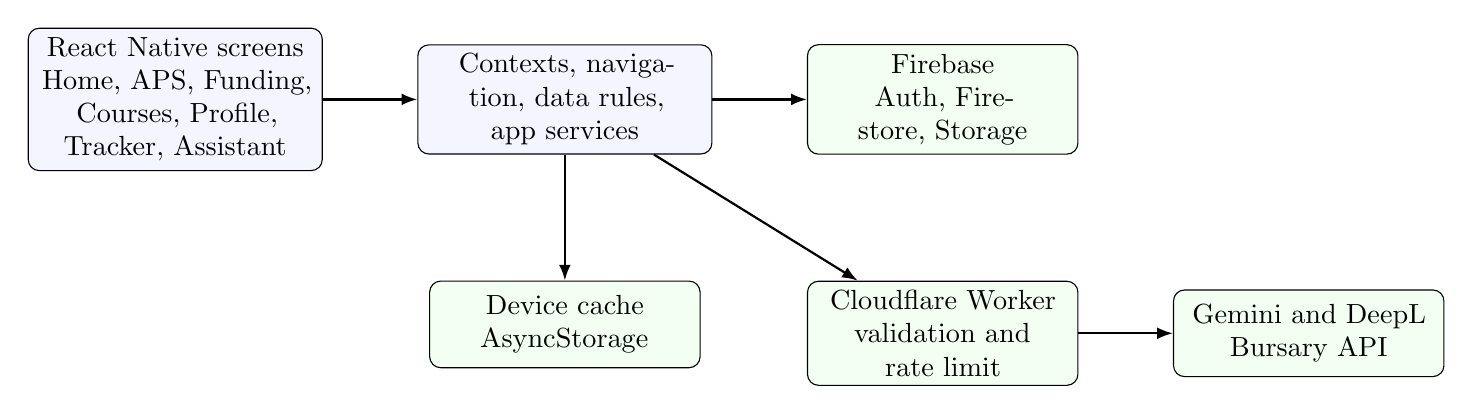
\begin{tikzpicture}[box/.style={draw,rounded corners,align=center,text width=35mm,minimum height=12mm,fill=blue!4},svc/.style={draw,rounded corners,align=center,text width=32mm,minimum height=11mm,fill=green!5},arr/.style={-{Latex[length=2mm]},thick}]
\node[box] (ui) {React Native screens\\Home, APS, Funding, Courses, Profile, Tracker, Assistant};
\node[box,right=12mm of ui] (logic) {Contexts, navigation, data rules, app services};
\node[svc,right=12mm of logic] (firebase) {Firebase\\Auth, Firestore, Storage};
\node[svc,below=16mm of logic] (cache) {Device cache\\AsyncStorage};
\node[svc,below=16mm of firebase] (worker) {Cloudflare Worker\\validation and rate limit};
\node[svc,right=12mm of worker] (api) {Gemini and DeepL\\Bursary API};
\draw[arr] (ui) -- (logic);
\draw[arr] (logic) -- (firebase);
\draw[arr] (logic) -- (cache);
\draw[arr] (logic) -- (worker);
\draw[arr] (worker) -- (api);
\end{tikzpicture}
\end{center}
The bursary endpoint is called directly by app code; assistant/translation secrets are kept behind the Worker.

\subsection{Code directory}
\begin{description}[style=nextline]
\item[\texttt{screens/}] App screens and Firebase initialization/authentication helpers.
\item[\texttt{components/}] Reusable cards, navigation elements, and shared UI.
\item[\texttt{navigation/}] Bottom tabs for Home, Funding, Universities, Courses, and Profile.
\item[\texttt{context/}] Profile/session, bookmarks, and language state providers.
\item[\texttt{data/}] Institution/course datasets, APS rules and matching, funding normalization, and local assistant knowledge.
\item[\texttt{services/}] APS scoring, career assessment persistence, notifications, translation, and requirements.
\item[\texttt{translation-worker/}] Cloudflare Worker source for assistant and translation routes.
\item[\texttt{assets/}] App branding and institution/college images.
\item[\texttt{docs/}] Design, status, and handoff documentation.
\end{description}

\section{Object-oriented domain model}
This UML-style model is a conceptual view over Firestore documents and local datasets. It does not claim that Firestore itself is relational.
\begin{center}
\resizebox{\textwidth}{!}{%
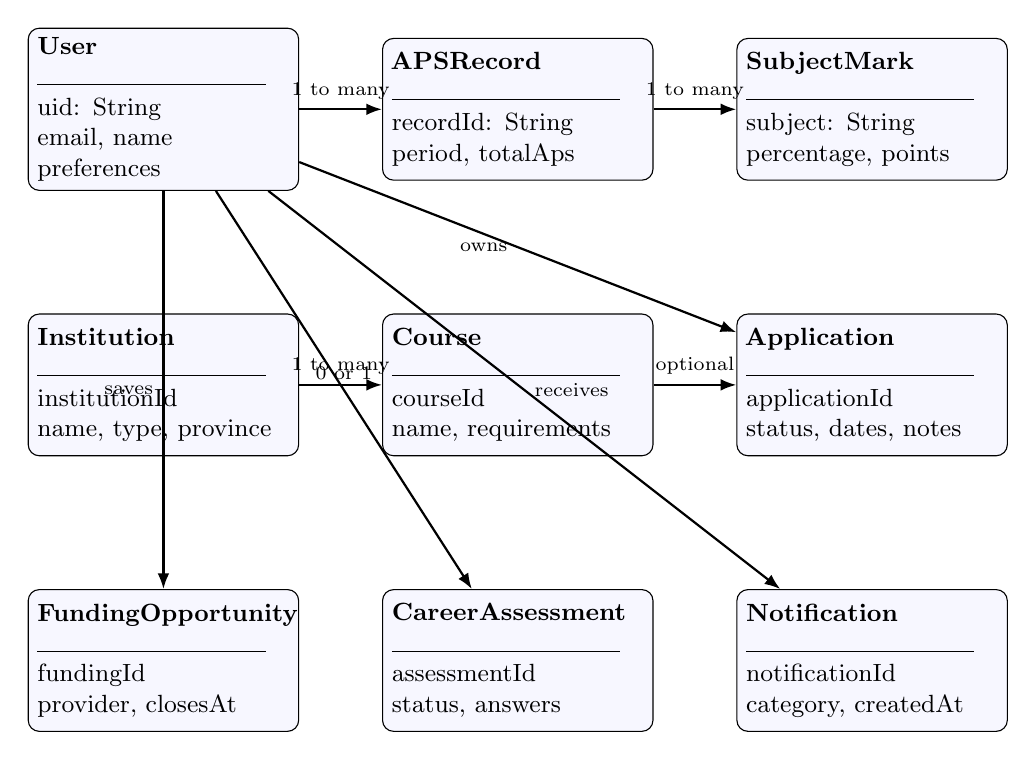
\begin{tikzpicture}[cls/.style={draw,rounded corners,align=left,text width=32mm,minimum height=18mm,font=\small,fill=blue!3},rel/.style={-{Latex[length=2mm]},thick}]
\node[cls] (user) at (0,5) {\textbf{User}\\\rule{29mm}{0.3pt}\\uid: String\\email, name\\preferences};
\node[cls] (aps) at (4.5,5) {\textbf{APSRecord}\\\rule{29mm}{0.3pt}\\recordId: String\\period, totalAps};
\node[cls] (mark) at (9,5) {\textbf{SubjectMark}\\\rule{29mm}{0.3pt}\\subject: String\\percentage, points};
\node[cls] (inst) at (0,1.5) {\textbf{Institution}\\\rule{29mm}{0.3pt}\\institutionId\\name, type, province};
\node[cls] (course) at (4.5,1.5) {\textbf{Course}\\\rule{29mm}{0.3pt}\\courseId\\name, requirements};
\node[cls] (app) at (9,1.5) {\textbf{Application}\\\rule{29mm}{0.3pt}\\applicationId\\status, dates, notes};
\node[cls] (fund) at (0,-2) {\textbf{FundingOpportunity}\\\rule{29mm}{0.3pt}\\fundingId\\provider, closesAt};
\node[cls] (assess) at (4.5,-2) {\textbf{CareerAssessment}\\\rule{29mm}{0.3pt}\\assessmentId\\status, answers};
\node[cls] (notice) at (9,-2) {\textbf{Notification}\\\rule{29mm}{0.3pt}\\notificationId\\category, createdAt};
\draw[rel] (user) -- node[above,font=\scriptsize]{1 to many} (aps);
\draw[rel] (aps) -- node[above,font=\scriptsize]{1 to many} (mark);
\draw[rel] (inst) -- node[above,font=\scriptsize]{1 to many} (course);
\draw[rel] (user) -- node[left,font=\scriptsize]{owns} (app);
\draw[rel] (course) -- node[above,font=\scriptsize]{optional} (app);
\draw[rel] (user) -- node[left,font=\scriptsize]{saves} (fund);
\draw[rel] (user) -- node[above,font=\scriptsize]{0 or 1} (assess);
\draw[rel] (user) -- node[right,font=\scriptsize]{receives} (notice);
\end{tikzpicture}}
\end{center}
Users can save many institutions, courses, and funding opportunities. The relational projection below represents these links with association tables. Institution-specific admission rules are associated with courses and an admissions year. Some APS rules are provisional or require verification.

\section{Categorized use cases}
\begin{longtable}{p{0.19\textwidth}p{0.25\textwidth}p{0.48\textwidth}}
\toprule
\textbf{Category} & \textbf{Use case} & \textbf{Actor and outcome}\\
\midrule
Account & Register/sign in & Learner authenticates; Firebase establishes the session.\\
Account & Edit profile & Authenticated learner updates profile fields persisted in the user record.\\
Account & Sign out/delete account & Learner ends session or requests permanent deletion after provider reauthentication.\\
Discovery & Browse institutions & Learner searches institutions and reviews their profiles.\\
Discovery & Browse courses & Learner reviews course details, requirements, and links.\\
APS planning & Calculate generic APS & Learner enters marks and receives the configured best-six estimate excluding Life Orientation.\\
APS planning & Compare institution rules & Learner reviews configured institution estimates and verification notes.\\
Funding & Find and save funding & Learner checks bursary details, closing dates, eligibility notes, and official links.\\
Applications & Track an application & Learner creates, updates, reviews, and deletes a personal application record.\\
Applications & Follow application guide & Learner reviews steps and institution-specific next actions.\\
Career planning & Complete assessment & Learner saves draft answers and reviews assessment results.\\
Notifications & Review notices/deadlines & Learner reads shared/personal notices and configured university/funding deadlines.\\
Assistant & Ask a question & Learner sends a question via Worker to Gemini; selected local answers support offline use.\\
Accessibility & Use voice tools & Learner uses speech recognition and text-to-speech after granting permissions.\\
Preferences & Change theme/language & Learner changes display and language preferences.\\
\bottomrule
\end{longtable}

\section{Logical relational model}
The app uses document-oriented Firestore. This normalized model is included because the assignment explicitly asks for a relational model; it is a conceptual projection, not a claim these SQL tables exist in production.
\begin{longtable}{p{0.25\textwidth}p{0.68\textwidth}}
\toprule
\textbf{Relation} & \textbf{Attributes (PK primary key; FK foreign key)}\\
\midrule
USER & user\_id PK, email, first\_name, surname, phone, photo\_url, auth\_provider, theme\\
INSTITUTION & institution\_id PK, name, institution\_type, province, website\_url, application\_url\\
COURSE & course\_id PK, institution\_id FK, name, faculty, qualification, description, prospectus\_url\\
ADMISSION\_RULE & rule\_id PK, course\_id FK, admissions\_year, method, minimum\_score, required\_subjects, verification\_status, source\_url\\
APS\_RECORD & aps\_record\_id PK, user\_id FK, period, total\_aps, created\_at\\
APS\_SUBJECT\_MARK & aps\_record\_id FK, subject\_name, percentage, points; composite PK (aps\_record\_id, subject\_name)\\
APPLICATION & application\_id PK, user\_id FK, institution\_id FK, course\_id FK nullable, status, submitted\_at, deadline, notes, updated\_at\\
FUNDING\_OPPORTUNITY & funding\_id PK, provider, title, description, eligibility, value, closes\_at, apply\_url, source\_url, last\_checked\\
UNIVERSITY\_BOOKMARK & user\_id FK, institution\_id FK; composite PK (user\_id, institution\_id)\\
COURSE\_BOOKMARK & user\_id FK, course\_id FK; composite PK (user\_id, course\_id)\\
FUNDING\_BOOKMARK & user\_id FK, funding\_id FK; composite PK (user\_id, funding\_id)\\
CAREER\_ASSESSMENT & assessment\_id PK, user\_id FK UNIQUE, status, answers, draft\_answers, version, started\_at, completed\_at\\
NOTIFICATION & notification\_id PK, user\_id FK nullable, category, title, body, route, created\_at, read\_at\\
\bottomrule
\end{longtable}

\subsection{Firestore paths observed in source}
\begin{itemize}
\item users collection documents store profile fields, bookmark ID arrays, and preference/status fields.
\item Each user's applications subcollection stores application tracker records.
\item careerAssessments documents store assessment records; local storage supports drafts/offline fallback.
\item Shared collections loaded by name include universities, colleges, courses, FAQs, applicationDeadlines, and notifications; the content loader caches fetched records locally.
\item Each user's notifications subcollection stores personal notifications; a notificationReads subcollection tracks shared notice read states.
\item Funding opportunities are fetched from an external API and cached in AsyncStorage; NSFAS has a built-in record.
\end{itemize}
Firebase Security Rules and live collection contents must be inspected in Firebase Console; source code cannot verify deployed rules or data.

\section{Screen flows and low-fidelity layouts}
\subsection{Primary learner flows}
\begin{center}
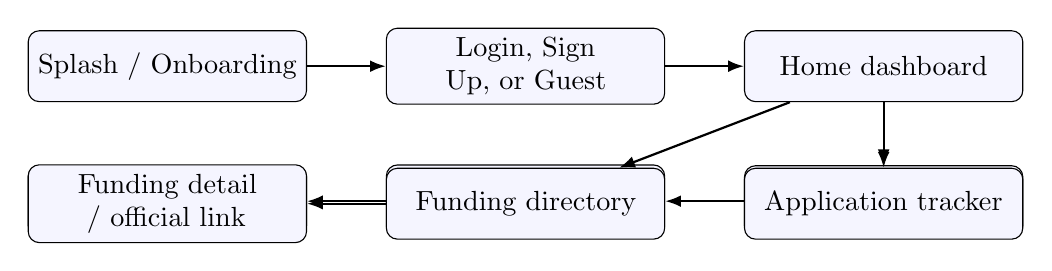
\begin{tikzpicture}[node distance=8mm and 10mm,flowbox/.style={draw,rounded corners,align=center,text width=33mm,minimum height=9mm,fill=blue!4},arr/.style={-{Latex[length=2mm]},thick}]
\node[flowbox] (start) {Splash / Onboarding};
\node[flowbox,right=of start] (login) {Login, Sign Up, or Guest};
\node[flowbox,right=of login] (home) {Home dashboard};
\node[flowbox,below=of home] (aps) {APS calculator};
\node[flowbox,left=of aps] (match) {Institution/course matches};
\node[flowbox,left=of match] (detail) {Course or institution details};
\node[flowbox,below=of login] (fund) {Funding directory};
\node[flowbox,left=of fund] (funddetail) {Funding detail / official link};
\node[flowbox,right=of fund] (tracker) {Application tracker};
\draw[arr] (start) -- (login);
\draw[arr] (login) -- (home);
\draw[arr] (home) -- (aps);
\draw[arr] (aps) -- (match);
\draw[arr] (match) -- (detail);
\draw[arr] (home) -- (fund);
\draw[arr] (fund) -- (funddetail);
\draw[arr] (home) -- (tracker);
\end{tikzpicture}
\end{center}

\subsection{Learner and service-connection sketch}
This conceptual sketch shows a learner using the mobile app to plan study options while the app reads reference information and calls online services. It is illustrative rather than a photograph or a record of a completed test.
\begin{center}
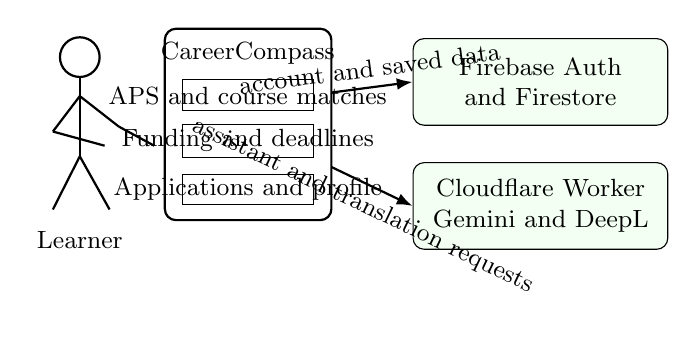
\begin{tikzpicture}[scale=0.9,every node/.style={font=\small},svc/.style={draw,rounded corners,align=center,text width=30mm,minimum height=11mm,fill=green!5},arr/.style={-{Latex[length=2mm]},thick}]
% Learner figure
\draw[thick] (0,3.6) circle (0.28);
\draw[thick] (0,3.32) -- (0,2.2);
\draw[thick] (0,3.05) -- (-0.38,2.55);
\draw[thick] (-0.38,2.55) -- (0.35,2.35);
\draw[thick] (0,3.05) -- (0.55,2.62);
\draw[thick] (0.55,2.62) -- (1.05,2.35);
\draw[thick] (0,2.2) -- (-0.38,1.45);
\draw[thick] (0,2.2) -- (0.42,1.45);
\node[below] at (0,1.28) {Learner};
% Mobile screen sketch
\draw[rounded corners,thick] (1.2,1.3) rectangle (3.55,4.0);
\node[align=center] at (2.37,3.65) {CareerCompass};
\draw (1.45,3.28) rectangle (3.3,2.85);
\node[align=center] at (2.37,3.06) {APS and course matches};
\draw (1.45,2.65) rectangle (3.3,2.18);
\node[align=center] at (2.37,2.42) {Funding and deadlines};
\draw (1.45,1.95) rectangle (3.3,1.52);
\node[align=center] at (2.37,1.73) {Applications and profile};
\node[svc] (cloud) at (6.5,3.25) {Firebase Auth and Firestore};
\node[svc] (worker) at (6.5,1.5) {Cloudflare Worker Gemini and DeepL};
\draw[arr] (3.55,3.1) -- node[above,sloped]{account and saved data} (cloud.west);
\draw[arr] (3.55,2.05) -- node[below,sloped]{assistant and translation requests} (worker.west);
\end{tikzpicture}
\end{center}

\subsection{Illustrative screen sketches}
These are design sketches, not screenshots of the current application. Replace or supplement them with legible screenshots from a running mobile device.
\noindent
\fbox{\begin{minipage}[t]{0.43\textwidth}
\textbf{Home}\par\smallskip
CareerCompass -- Welcome, Learner\par
[View my APS] [Find funding]\par
APS course matches: 4\par
Upcoming deadlines\par
[Institution card] [Bursary card]\par
Home | Funding | Institutions | Courses | Profile
\end{minipage}}
\hfill
\fbox{\begin{minipage}[t]{0.43\textwidth}
\textbf{APS Calculator}\par\smallskip
Period: Grade 12\par
Mathematics [78 percent]\par
English [82 percent]\par
[Add subject]\par
[Calculate] [Save]\par
Estimate and institution caveats
\end{minipage}}
\par\medskip
\noindent
\fbox{\begin{minipage}[t]{0.43\textwidth}
\textbf{Funding}\par\smallskip
Funding opportunities\par
[Search bursaries] [Filter]\par
[NSFAS card: closes/date]\par
[Bursary card: provider]\par
[Official details and apply link]
\end{minipage}}
\hfill
\fbox{\begin{minipage}[t]{0.43\textwidth}
\textbf{Application tracker}\par\smallskip
My applications\par
[Add application]\par
Institution / Course\par
Status / Deadline\par
Required next action\par
[Open] [Edit] [Delete]
\end{minipage}}

\section{Persistence, integrations, and security}
Firebase Authentication manages identity. User profiles/bookmarks are written to Firestore and cached locally. Applications are stored under each user's Firestore subcollection. Career assessments sync to Firestore with local draft/fallback behavior. Reference content loaded through the content loader is cached in AsyncStorage. Funding has a separate cache and NSFAS fallback. Offline behavior is partial: online assistant responses, API refreshes, and uncached remote records require connectivity.
\begin{itemize}
\item Firebase Authentication: email/password and Google sign-in.
\item Cloud Firestore: profiles, applications, assessments, shared content, and notifications.
\item Firebase Storage: profile-image handling where configured.
\item Cloudflare Worker: assistant and translation routes with request validation/rate limiting.
\item Gemini API: online assistant responses through the Worker.
\item DeepL API: translations through the Worker when configured.
\item Bursary API: external funding directory source.
\item Device speech services: speech recognition and text-to-speech.
\end{itemize}
\textbf{Security:} never put Gemini/DeepL secrets in app source, public client variables, screenshots, or this document. Configure them as Worker secrets. Firestore rules, OAuth fingerprints, and access controls require account-owner verification.

\section{Non-functional requirements and quality plan}
\begin{longtable}{p{0.18\textwidth}p{0.45\textwidth}p{0.29\textwidth}}
\toprule
\textbf{Attribute} & \textbf{Design response} & \textbf{Evidence to collect}\\
\midrule
Usability & Mobile-first cards, search/filter, navigation, and accessibility labels. & New-learner task walkthrough and screenshots.\\
Availability & Cached content and local assistant fallback. & Disable Wi-Fi, cold start, inspect cached screens and error states.\\
Performance & Asynchronous data loads and API timeouts. & Measure launch, directory load, and assistant response on device.\\
Maintainability & Screens, components, contexts, services, and data rules are separated. & Explain code map and lint result.\\
Modifiability & APS rules and normalized data are separated from UI rendering. & Demonstrate changing a rule without duplicating screen logic.\\
Scalability & Firestore and a server-side proxy provide paths for shared data and secret-backed services. & Verify rules, indexes, quotas, and rate limits.\\
Resilience & Caches, validation, error handling, and lifecycle logging exist in source. & Test offline, restart, denied permissions, expired auth, and recovery.\\
Compatibility & Expo/React Native with app-config plugins for native permissions. & Fresh APK on a physical Android device and screen-size checks.\\
\bottomrule
\end{longtable}

\section{CRUD and coursework evidence checklist}
The source contains create/read/update/delete paths, but assessment evidence must be captured from the real app and Firebase Console:
\begin{enumerate}
\item Create a test account and an application tracker record; save marks/assessment data.
\item Read the profile, applications, bookmarks, and reference content after sign-in/restart.
\item Update a profile field and application status; show the saved value after navigating away.
\item Delete a test application; use only a disposable account to demonstrate permanent account deletion.
\item Capture Firebase collection/document structure and rules without exposing personal data or credentials.
\item Capture repository/class organization and version-control history.
\end{enumerate}

\section{Lifecycle, debugging, profiling, and functional demonstration}
The brief requires evidence, not just a description. Assemble the following from the actual environment:
\begin{itemize}
\item install a fresh build on a physical device and record device, OS, and build version;
\item set a breakpoint in a screen/service, step through, and capture variable state;
\item capture CPU or memory profiling from Android Studio or another permitted profiler;
\item capture logs for app start, background, resume, and termination/reopen;
\item demonstrate sign in, APS calculation, course inspection, bookmarking, tracker CRUD, and an official funding/application link;
\item repeat selected flows offline and with permissions denied.
\end{itemize}
No device screenshots or completed profiler/debugging evidence were supplied for this document. Add authentic dated evidence before marking these checkpoints complete.

\section{Limitations and verification items}
\begin{itemize}
\item Institution course data, APS rules, deadlines, bursary eligibility, logos, and images require official source citations and periodic review. Some APS rules are provisional.
\item Firebase data quality and production Security Rules cannot be verified from client code alone.
\item Google sign-in needs testing with the EAS-signed Android build and correct Firebase OAuth fingerprints.
\item The online assistant depends on Gemini availability, Worker configuration, quota, connectivity, and the installed app build.
\item Current deadline reminders are local scheduled reminders; push notices while the app is closed require separate server infrastructure.
\item A secure document vault, verified bursary eligibility engine, and institution-side application submission are not claimed as implemented.
\end{itemize}

\section{Presentation outline}
The brief asks for introduction, problem, objectives, solution design, implementation, and system architecture. Suggested order:
\begin{enumerate}
\item Introduction, target learners, and study-planning problem.
\item Problem statement and measurable project objectives.
\item Design: domain model, use cases, relational projection, screen flows, and offline plan.
\item Implementation: Expo/React Native, Firebase, APS/funding data, Worker/Gemini, and device speech.
\item Real-device end-to-end and CRUD demonstration.
\item Quality, limitations, profiler/lifecycle evidence, and future work.
\end{enumerate}

\section{References}
\begin{enumerate}
\item Mabokela, K. R. (2025). \emph{DSW02B1 Group Project Practical Work}, University of Johannesburg. Supplied brief.
\item Expo documentation. \url{https://docs.expo.dev/}
\item Firebase documentation. \url{https://firebase.google.com/docs}
\item Cloudflare Workers documentation. \url{https://developers.cloudflare.com/workers/}
\item Google AI for Developers, Gemini API. \url{https://ai.google.dev/gemini-api/docs}
\item DeepL API documentation. \url{https://developers.deepl.com/docs}
\item Cite each institution, bursary, logo, image, and dataset source individually in the final submission, including source links and last-checked dates where available.
\end{enumerate}
\end{document}
